\documentclass{article}

%====================================================
%                  PACKAGES
%====================================================
\usepackage{graphicx}
\usepackage{subcaption}
\usepackage{fancyhdr}
\usepackage[margin=1in]{geometry}
\usepackage{listings}
\usepackage[hidelinks]{hyperref}
\usepackage{amsmath,amssymb,mathtools}
\usepackage{float}
\usepackage{lmodern}
\usepackage{xcolor}
\usepackage{fvextra}
\usepackage{longtable}
\usepackage{enumitem}
\usepackage{booktabs}
\usepackage{array}
\usepackage{multirow}
\usepackage{colortbl}
\usepackage{titlesec}
\usepackage{tikz}
\usepackage{eso-pic} % برای بک‌گراند صفحه اول
\usepackage[most]{tcolorbox}
\usepackage{xepersian}
\usetikzlibrary{calc} % اضافه شده برای محاسبات مختصات در tikz

%====================================================
%                  COLORS
%====================================================

\definecolor{mainblue}{RGB}{15,76,129}
\definecolor{lightblue}{RGB}{226,238,250}
\definecolor{deepblue}{RGB}{9,24,51} % تیره‌تر و پررنگ‌تر برای بک‌گراند
\definecolor{darkpurple}{RGB}{60,20,80} % بنفش تیره و پررنگ‌تر برای گرادیانت

\definecolor{mygreen}{RGB}{18,122,86}
\definecolor{softgreen}{RGB}{233,248,241}

\definecolor{softred}{RGB}{210,73,73}
\definecolor{softpink}{RGB}{252,236,239}

\definecolor{golden}{RGB}{255,204,0} % طلایی درخشان
\definecolor{softorange}{RGB}{255,244,224}

\definecolor{softgray}{RGB}{245,245,245}
\definecolor{glassbg}{RGB}{255,255,255} % تعریف رنگ سفید، شفافیت در tcolorbox اعمال می‌شود

%====================================================
%                  HYPERREF
%====================================================

\hypersetup{
	colorlinks=true,
	linkcolor=mainblue, % تغییر به mainblue برای هماهنگی بیشتر
	filecolor=magenta,
	urlcolor=mainblue, % تغییر به mainblue
	citecolor=mygreen % تغییر به mygreen
}


%====================================================
%                  FONTS
%====================================================

\settextfont[Path={./font/}, Scale=1.3]{IRLotus}
\setlatintextfont[Scale=1]{Times New Roman}

%====================================================
%                  PAGE STYLE
%====================================================

\setlength\headheight{28pt}
\pagestyle{fancy}
\fancyhf{}
\lhead{\textcolor{mainblue}{\textbf{تمرین چهارم}}}
\chead{
\includegraphics[width=1cm,height=1cm,keepaspectratio]{img/Logo.png}}
\rhead{\textcolor{mainblue}{\textbf{\thepage}}}
\rfoot{\textcolor{gray}{حامد بهروزی مقدم - آیدین صحنه - مانی وفاپور}}
\renewcommand{\headrulewidth}{1.5pt} % ضخیم‌تر کردن خط هدر
\renewcommand{\headrule}{\hbox to\headwidth{\color{mainblue}\leaders\hrule height \headrulewidth\hfill}}
\renewcommand{\footrulewidth}{1pt}
\renewcommand{\footrule}{\hbox to\headwidth{\color{gray}\leaders\hrule height \footrulewidth\hfill}}

%====================================================
%                  SECTION STYLE
%====================================================


\titleformat{\section}
{\Large\bfseries\color{mainblue}}
{\begin{tikzpicture}[baseline={(0,-0.1)}]
		\node[fill=mainblue,text=white,rounded corners=2pt,inner sep=4pt] {\thesection};
\end{tikzpicture}}
{0.5em}
{}[\vspace{0.2ex}\titlerule] % خط زیر عنوان

% اضافه کردن این خط برای تنظیم فاصله بعد از عنوان:
\titlespacing{\section}{0pt}{20pt}{10pt} % مقدار 10pt را کم یا زیاد کنید تا فاصله تنظیم شود

%====================================================
%                  LINE SPACING & LISTINGS
%====================================================

\renewcommand{\baselinestretch}{1.5}

\definecolor{codegreen}{rgb}{0,0.55,0}
\definecolor{codegray}{rgb}{0.45,0.45,0.45}
\definecolor{codepurple}{rgb}{0.58,0,0.82}
\definecolor{backcolour}{rgb}{0.97,0.97,0.94}

\lstdefinestyle{mystyle}{
	backgroundcolor=\color{backcolour},
	commentstyle=\color{codegreen},
	keywordstyle=\color{magenta},
	numberstyle=\tiny\color{codegray},
	stringstyle=\color{codepurple},
	basicstyle=\ttfamily\footnotesize,
	breakatwhitespace=false,
	breaklines=true,
	captionpos=b,
	keepspaces=true,
	numbers=left,
	numbersep=6pt,
	showspaces=false,
	showstringspaces=false,
	showtabs=false,
	tabsize=4,
	frame=shadowbox, % تغییر به shadowbox برای جلوه بهتر
	rulesepcolor=\color{mainblue}
}
\lstset{style=mystyle}

%====================================================
%                  TCOLORBOX
%====================================================

\tcbset{
	enhanced,
	breakable,
	arc=4mm, % گوشه‌های گردتر
	boxrule=1.2pt, % خط ضخیم‌تر
	fonttitle=\bfseries\large, % عنوان کادر بزرگتر و پررنگ‌تر
	drop fuzzy shadow % اضافه کردن سایه برای تمام tcolorbox ها
}

%====================================================
%                  AUTOREF
%====================================================

\AtBeginDocument{
	\def\chapterautorefname{فصل}%
	\def\sectionautorefname{بخش}%
	\def\subsectionautorefname{زیربخش}%
	\def\equationautorefname{رابطه}%
	\def\figureautorefname{شکل}%
	\def\tableautorefname{جدول}%
}

%====================================================
%                  DOCUMENT
%====================================================

\begin{document}
	
	%====================================================
	%                  TITLE PAGE
	%====================================================
	
	\begin{titlepage}
		% پس زمینه آبی تیره و سفید برای جداول و پس زمینه
		\AddToShipoutPictureBG*{
			\begin{tikzpicture}[remember picture,overlay]
				% بک‌گراند اصلی آبی تیره
				\fill[deepblue] (current page.south west) rectangle (current page.north east);
				% نوار گرادیانت سفید در بالای صفحه
				\shade[top color=white, bottom color=white, opacity=0.08] 
				(current page.north west) rectangle ($(current page.north east)+(0,-6cm)$);
				% اشکال هندسی محو به رنگ سفید
				\fill[white, opacity=0.03] (current page.north west) circle (8cm);
				\fill[white, opacity=0.02] (current page.south east) circle (12cm);
				\fill[white, opacity=0.04] (current page.north east) +(-4cm,-4cm) circle (6cm);
				\fill[white, opacity=0.03] (current page.south west) +(4cm,4cm) rectangle +(8cm,8cm);
				\fill[white, opacity=0.02] (current page.center) circle (5cm);
				
				% کادر بیرونی سفید
				\draw[white, ultra thick, rounded corners=15pt, opacity=0.7] 
				($(current page.north west)+(1.5cm,-1.5cm)$) rectangle ($(current page.south east)+(-1.5cm,1.5cm)$);
				% کادر داخلی خط‌چین سفید
				\draw[white, thick, dashed, opacity=0.2] 
				($(current page.north west)+(1.7cm,-1.7cm)$) rectangle ($(current page.south east)+(-1.7cm,1.7cm)$);
			\end{tikzpicture}
		}
		
		\begin{center}
			\vspace*{1.5cm} % کاهش فاصله
			
			{\fontsize{38}{42}\selectfont \textbf{\textcolor{white}{تمرین سری چهارم}}} % عنوان اصلی سفید با فونت بزرگتر
			
			\vspace{0.8cm} % کاهش فاصله
			
			{\LARGE \textbf{\textcolor{white}{یادگیری ماشین مقدماتی}}} % نام درس سفید
			
			\vspace{1cm} % کاهش فاصله
			
			% در صورتی که لوگو بک‌گراند سفید دارد، از فایل png بدون پس زمینه استفاده کنید
			\begin{tcolorbox}[
				colback=white,       % پس‌زمینه سفید
				colframe=white,      % بدون خط دور (یا می‌توانید رنگی انتخاب کنید)
				boxrule=0pt,         % ضخامت لبه‌ها صفر (بدون خط)
				arc=3mm,             % گردی گوشه‌ها (مطابق با سبک کادر اصلی)
				left=2mm, right=2mm, top=2mm, bottom=2mm, % فاصله داخلی
				width=0.2\textwidth, % عرض کادر (مطابق با چیزی که قبلا داشتید)
				halign=center        % وسط‌چین کردن لوگو در کادر
				]
				
\includegraphics[width=\linewidth]{img/Logo.png}
			\end{tcolorbox}
			
			\vspace{1.2cm} % کاهش فاصله
			
			\begin{tcolorbox}[
				width=0.85\textwidth,
				colback=white, % پس‌زمینه سفید
				opacityback=0.1, % شفافیت سفید برای هماهنگی با بک‌گراند آبی
				colframe=white, % فریم سفید
				coltitle=deepblue, % رنگ عنوان کادر آبی تیره
				title={\centering \Large \textbf{\textcolor{deepblue}{GAN/VAE}}}, % متن عنوان کادر آبی تیره
				halign=center,
				arc=5mm, % گوشه‌های گردتر
				boxrule=1.5pt, % خط ضخیم‌تر
				shadow={2mm}{-2mm}{0mm}{black!40} % سایه جذاب
				]
				\large
				\textcolor{deepblue}{بررسی عملکرد مدل‌های VAE و cDCGAN در بازسازی و بهبود توازن مجموعه‌داده‌های تصویری}
			\end{tcolorbox}
			
			\vspace{1cm} % کاهش فاصله
			
			% جدول مشخصات با پس‌زمینه سفید و متن آبی
			\begin{tcolorbox}[
				width=0.75\textwidth,
				colback=white, % پس‌زمینه سفید
				colframe=white, % فریم سفید
				arc=3mm,
				boxrule=2pt,
				halign=center,
				shadow={1mm}{-1mm}{0mm}{black!20} % سایه ملایم
				]
				\renewcommand{\arraystretch}{1.5} % کاهش برای جا شدن در صفحه اول
				\large
				\begin{tabular}{>{\bfseries\color{mainblue}}l l} % عنوان‌ها پررنگ و آبی
					نام دانشجو: & حامد بهروزی مقدم - آیدین صحنه - مانی وفاپور \\
					شماره دانشجویی: & 40215633 - 40120243 - 40123783 \\
					استاد درس: & دکتر نیکوفرد  \\
					نیمسال: & 1404-1405 \\
				\end{tabular}
			\end{tcolorbox}
			
		\end{center}
	\end{titlepage}
	
	%====================================================
	%                  TABLE OF CONTENTS
	%====================================================
	
	\tableofcontents
	\clearpage
	
\section{سوال 1}
\subsection{تحلیل نتایج بخش ۱-۱ (بارگذاری داده‌ها و آموزش شبکه \lr{ResNet})}

پس از آماده‌سازی مجموعه داده‌ی \lr{BreastMNIST} و بازآموزی (\lr{Fine-tuning}) مدل پیش‌آموزش‌دیده‌ی \lr{ResNet-18} برای ۵ دوره (\lr{Epoch})، نتایج به دست آمده در دو بخش «روند آموزش» و «ماتریس آشفتگی» قابل ارزیابی است:

\vspace{0.5cm}
\textbf{۱. تحلیل نمودار روند آموزش و پدیده بیش‌برازش (\lr{Overfitting}):}

با بررسی لاگ‌های خروجی و نمودار دقت (\lr{Accuracy vs. Epochs})، مشاهده می‌شود که دقت مدل روی داده‌های آموزشی بسیار سریع افزایش یافته و در دوره‌های سوم تا پنجم به نزدیکی ۱۰۰٪ (حدود ۹۹٫۸۲٪) رسیده است. با این حال، دقت اعتبارسنجی (\lr{Validation Accuracy}) نتوانسته همگام با دقت آموزش رشد کند و در حدود ۸۸٪ متوقف شده و حتی در دوره‌ی پنجم با افت جزئی مواجه شده است. 

این فاصله‌ی معنادار (\lr{Gap}) بین دقت آموزش و اعتبارسنجی، نشان‌دهنده‌ی وقوع پدیده‌ی \textbf{بیش‌برازش (\lr{Overfitting})} است. از آنجایی که معماری \lr{ResNet-18} ظرفیت یادگیری بالایی دارد و مجموعه داده‌ی \lr{BreastMNIST} شامل تعداد بسیار کمی تصویر (تنها ۵۴۶ تصویر آموزشی) است، شبکه به جای یادگیری الگوهای تعمیم‌پذیر، اقدام به حفظ کردن داده‌های آموزشی کرده است.

\begin{figure}[H]
	\centering
	% نام فایل تصویر نمودار دقت خود را در خط زیر جایگزین کنید
	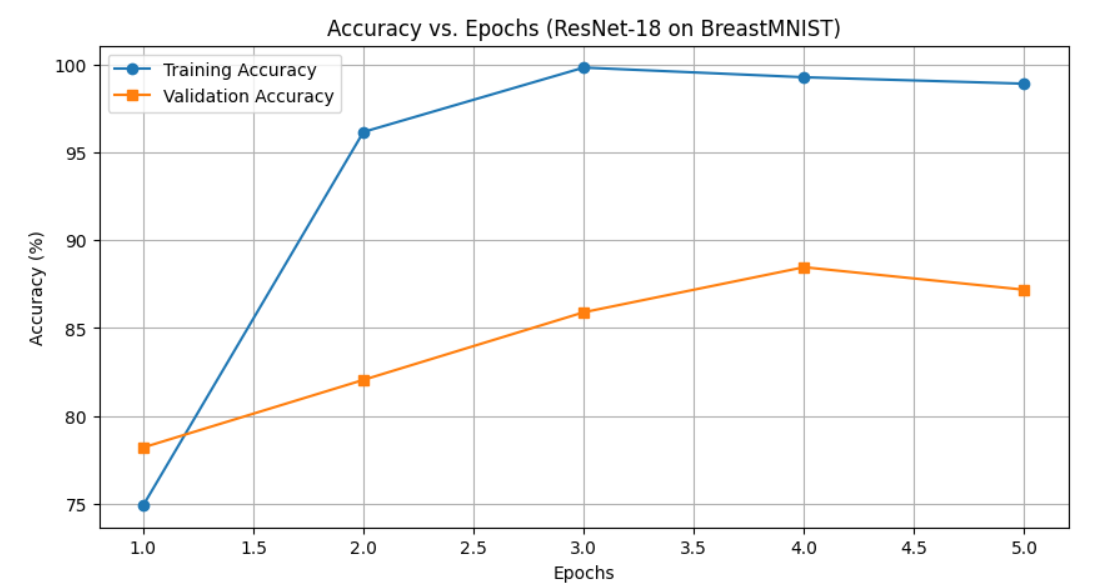
\includegraphics[width=0.75\textwidth]{accuracy_plot.png} 
	\caption{نمودار دقت آموزش و اعتبارسنجی بر حسب دوره‌ها}
	\label{fig:resnet_accuracy}
\end{figure}

\vspace{0.5cm}
\textbf{۲. تحلیل ماتریس آشفتگی و مشکل نامتوازن بودن کلاس‌ها (\lr{Class Imbalance}):}

دقت نهایی مدل روی داده‌های تست ۸۲٫۶۹٪ گزارش شده است. اگرچه این عدد در نگاه اول قابل قبول به نظر می‌رسد، اما بررسی \textbf{ماتریس آشفتگی (\lr{Confusion Matrix})} یک مشکل اساسی را آشکار می‌کند:

\begin{itemize}
	\item مدل در تشخیص کلاس ۱ (\lr{Normal/Benign} - سالم/خوش‌خیم) عملکرد بسیار خوبی داشته و از ۱۱۴ نمونه، ۱۰۸ مورد را به درستی تشخیص داده است.
	\item اما در تشخیص کلاس ۰ (\lr{Malignant} - بدخیم)، مدل به شدت ضعیف عمل کرده است؛ به طوری که از ۴۲ نمونه‌ی بدخیم، نیمی از آن‌ها (۲۱ مورد) را به اشتباه سالم تشخیص داده است (نرخ بالای \lr{False Negative}).
\end{itemize}

\begin{figure}[H]
	\centering
	% نام فایل تصویر ماتریس آشفتگی خود را در خط زیر جایگزین کنید
	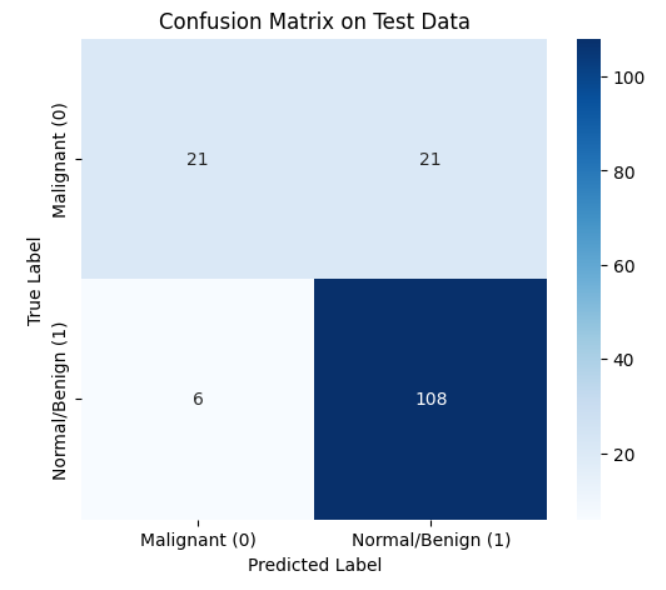
\includegraphics[width=0.6\textwidth]{confusion_matrix.png} 
	\caption{ماتریس آشفتگی مدل \lr{ResNet-18} روی داده‌های تست}
	\label{fig:resnet_cm}
\end{figure}

\vspace{0.5cm}
\textbf{نتیجه‌گیری این بخش:}

در مسائل پردازش تصاویر پزشکی، تشخیص اشتباهِ یک تومور بدخیم به عنوان بافت سالم (\lr{False Negative}) هزینه‌ی جانی در پی دارد. عملکرد ضعیف مدل در کلاس ۰ مستقیماً ناشی از \textbf{توزیع نامتوازن داده‌ها} در مجموعه داده‌ی اولیه است (تعداد داده‌های سالم بسیار بیشتر از بدخیم است). شبکه به دلیل مشاهده‌ی بیشترِ کلاس سالم، به سمت انتخاب این کلاس سوگیری (\lr{Bias}) پیدا کرده است. این نتایج، ضرورت استفاده از تکنیک‌های تولید داده (مانند شبکه‌های متخاصم مولد - \lr{GAN}) برای افزایش تعداد نمونه‌های کلاس اقلیت و رفع مشکل نامتوازنی را به وضوح توجیه می‌کند.


\subsection{تحلیل نتایج بخش ۱-۲ (شبکه \lr{Conditional DCGAN})}

در این بخش، یک شبکه \lr{Conditional DCGAN} برای تولید نمونه‌های مصنوعی آموزش داده شد. استفاده از تکنیک‌های پایدارسازی در این مدل، منجر به نتایج زیر شد:

\vspace{0.5cm}
\textbf{الف- تحلیل ساختار و پارامترهای شبکه:}

شبکه مولد (\lr{Generator}) دارای \lr{1,079,717} پارامتر و شبکه تفکیک‌کننده (\lr{Discriminator}) دارای \lr{141,409} پارامتر است. این عدم تقارن ساختاری (بزرگتر بودن مولد به نسبت تقریباً ۷٫۶ برابر)، یک انتخاب معماریِ آگاهانه است. از آنجایی که نگاشتِ یک بردار نویز تصادفی ($z$) به فضای پیچیده‌ی تصاویر پزشکی نیازمند ظرفیت بازنمایی (\lr{Representational Capacity}) بالایی است، شبکه مولد عمیق‌تر طراحی شده است.

\vspace{0.5cm}
\textbf{ب- تفسیر نمودار \lr{Loss} شبکه‌های مولد و تفکیک‌کننده:}

نمودار خطای ثبت شده در ۵۰ دوره، نمایانگر یک رقابت زنده و رسیدن به مجاورت یک «تعادل نش» (\lr{Nash Equilibrium}) است.
در ۳۰ دوره‌ی ابتدایی، خطای تفکیک‌کننده روند نزولی داشته و به کمینه خود رسید، در حالی که خطای مولد افزایش یافت. اما نکته‌ی کلیدی از دوره‌ی ۳۰ به بعد رخ داد؛ جایی که یک چرخش (\lr{Reversal}) در نمودارها مشاهده می‌شود. خطای تفکیک‌کننده مجدداً افزایش یافته و خطای مولد با شیب تندی کاهش می‌یابد. این رفتارِ نوسانی اثبات می‌کند که مولد توانسته است در دوره‌های پایانی، ویژگی‌های توزیع داده‌ها را به خوبی مدل‌سازی کند.

\begin{figure}[H]
	\centering
	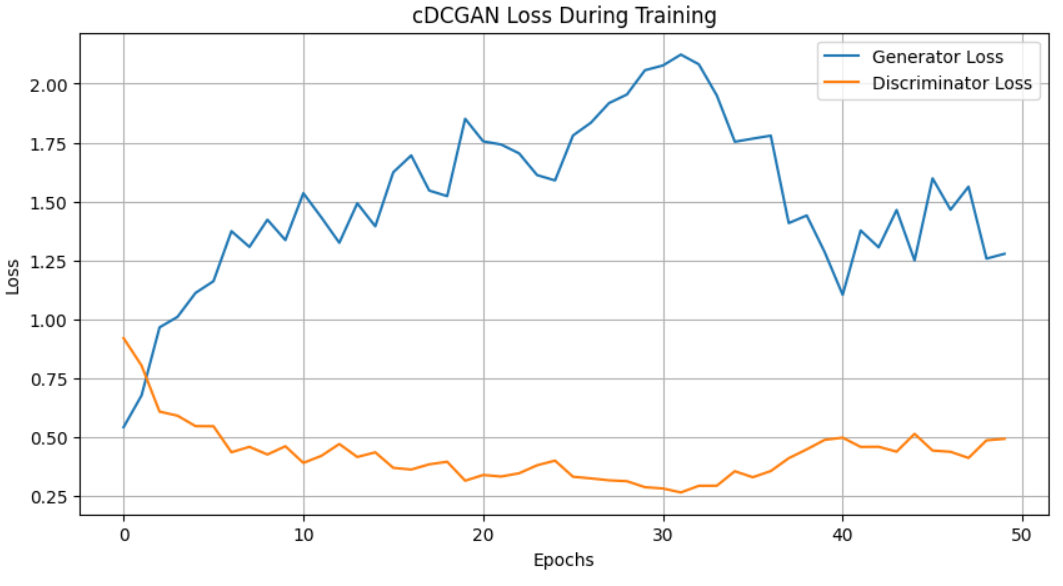
\includegraphics[width=0.7\textwidth]{loss_plot.png} 
	\caption{نمودار تغییرات تابع هزینه (\lr{Loss}) برای دو شبکه مولد و تفکیک‌کننده}
	\label{fig:gan_loss}
\end{figure}

\vspace{0.5cm}
\textbf{پ- تحلیل نمونه‌های تولید شده:}

تصاویر تولید شده نشان‌دهنده‌ی شکل‌گیری ساختار کلی بافت‌ها هستند. تأثیر شرطی‌سازی (\lr{Conditioning}) در اینجا مشهود است، زیرا بافت کلی تصاویر در دو کلاس تفاوت‌های ظریفی با یکدیگر دارند. با این وجود، شباهت‌های ساختاری درون‌کلاسی، نشان‌دهنده وقوع یک «فروپاشی حالتِ خفیف» (\lr{Mild Mode Collapse}) است که در آموزش کوتاه‌مدتِ شبکه‌های \lr{GAN} روی توزیع‌های پیچیده‌ی پزشکی طبیعی است.

\begin{figure}[H]
	\centering
	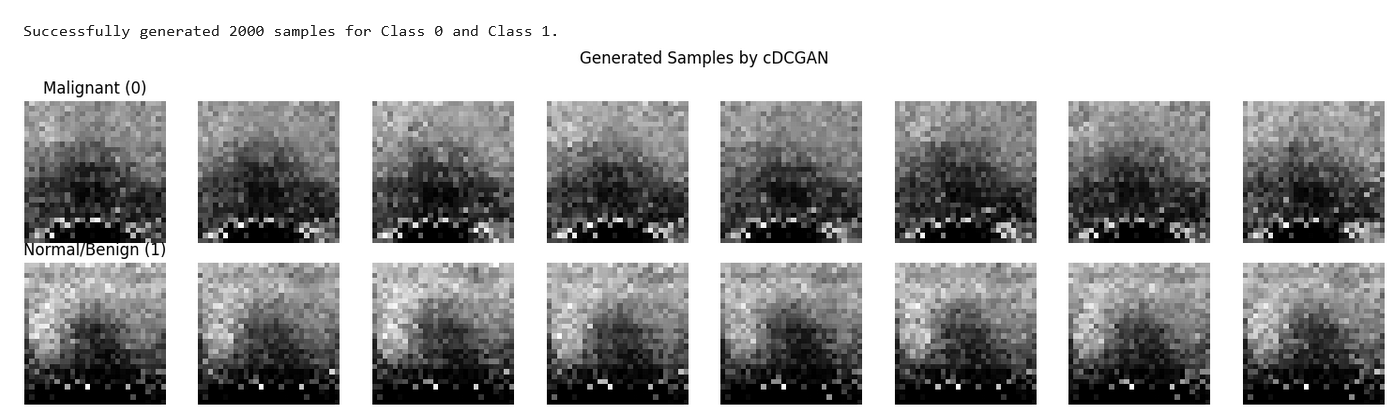
\includegraphics[width=0.8\textwidth]{generated_samples.png} 
	\caption{نمونه تصاویر تولید شده توسط مولد برای کلاس‌های بدخیم و سالم}
	\label{fig:gan_samples}
\end{figure}

\vspace{0.5cm}
\textbf{ت- بررسی اثربخشی راهکارهای پایدارسازی:}

برای جلوگیری از فروپاشی شبکه، دو رویکرد زیر اعمال شد که اثربخشی آن‌ها در نمودارها مشهود است:
\begin{enumerate}
	\item \textbf{قاعده به‌روزرسانی دو مقیاس زمانی (\lr{TTUR}):} با تنظیم نرخ یادگیری تفکیک‌کننده روی مقدار کمتر از مولد ($\alpha_D = 0.00005$ در برابر $\alpha_G = 0.0002$)، سرعت همگرایی تفکیک‌کننده کنترل شد.
	\item \textbf{هموارسازی برچسب‌ها (\lr{One-sided Label Smoothing}):} با جایگزینی مقدار $1.0$ با $0.9$ برای تصاویر واقعی، از اطمینان بیش از حد (\lr{Overconfidence}) تفکیک‌کننده و در نتیجه محو شدن گرادیان جلوگیری شد.
\end{enumerate}






\subsection{تحلیل و مقایسه نتایج طبقه‌بندی با کمک داده‌های مولد (بخش ۱-۳)}

در این بخش، مجموعه داده‌ی آموزشی با استفاده از نمونه‌های تولید شده توسط شبکه‌ی \lr{cDCGAN} متوازن شد (۱۰۰۰ نمونه برای هر کلاس) و شبکه \lr{ResNet-18} مجدداً از صفر روی این داده‌های ترکیبی آموزش دید. مقایسه نتایج این بخش با نتایج بخش اول (بدون استفاده از داده‌های مصنوعی) دستاوردهای مهم زیر را نشان می‌دهد:

\vspace{0.5cm}
\textbf{۱. بهبود چشمگیر در دقت کلی و تعمیم‌پذیری (\lr{Generalization}):}

دقت نهایی مدل روی داده‌های تست (\lr{Test Accuracy}) از ۸۲٫۶۹٪ در بخش اول، به ۸۸٫۴۶٪ در این بخش افزایش یافته است. این ارتقای تقریباً ۶ درصدی نشان می‌دهد که تزریق داده‌های تولید شده توسط \lr{GAN}، نه تنها باعث سردرگمی مدل نشده، بلکه با فراهم کردن تنوع بیشتر در ویژگی‌های تصاویر، توانایی مدل را در تعمیمِ الگوها به داده‌های جدید (داده‌های تست) به شدت بالا برده است.

\vspace{0.5cm}
\textbf{۲. رفع مشکل سوگیری (\lr{Bias}) و بهبود تشخیص کلاس اقلیت:}

مهم‌ترین نتیجه‌ی این آزمایش با مقایسه‌ی ماتریس‌های آشفتگی (\lr{Confusion Matrices}) در دو حالت به دست می‌آید. در مسائل پزشکی، تشخیص درست کلاس بدخیم (\lr{Malignant - Class 0}) حیاتی‌ترین وظیفه‌ی مدل است:
\begin{itemize}
	\item \textbf{در بخش اول (داده‌های نامتوازن):} شبکه به دلیل کمبود داده‌های کلاس بدخیم، سوگیری شدیدی به سمت کلاس سالم داشت. به طوری که از ۴۲ نمونه‌ی بدخیم، نیمی از آن‌ها (۲۱ مورد) را به اشتباه سالم تشخیص داده بود.
	\item \textbf{در این بخش (داده‌های متوازن شده با \lr{GAN}):} با جبران کمبود داده‌ها، قدرت مدل در تشخیص تومورهای بدخیم به شکل خیره‌کننده‌ای افزایش یافت. خطای تشخیص در این کلاس حساس از ۲۱ مورد به تنها ۱۰ مورد کاهش یافت و مدل توانست ۳۲ مورد را به درستی تشخیص دهد.
\end{itemize}

\vspace{0.5cm}
\textbf{۳. حفظ پایداری در تشخیص کلاس اکثریت:}

با وجود اینکه تمرکز شبکه روی یادگیری کلاس بدخیم بیشتر شد، اما مدل توانست عملکرد عالی خود را در تشخیص بافت‌های سالم/خوش‌خیم (\lr{Normal/Benign - Class 1}) حفظ کند (کاهش بسیار ناچیز از ۱۰۸ تشخیص درست به ۱۰۶ تشخیص درست از مجموع ۱۱۴ داده). این نشان می‌دهد که ما با پدیده فراموشی فاجعه‌بار مواجه نشدیم و مدل یک مرز تصمیم‌گیری (\lr{Decision Boundary}) بسیار دقیق‌تر بین دو کلاس رسم کرده است.

\begin{figure}[H]
	\centering
	% نام فایل تصویر ماتریس آشفتگی جدید خود را در خط زیر جایگزین کنید
	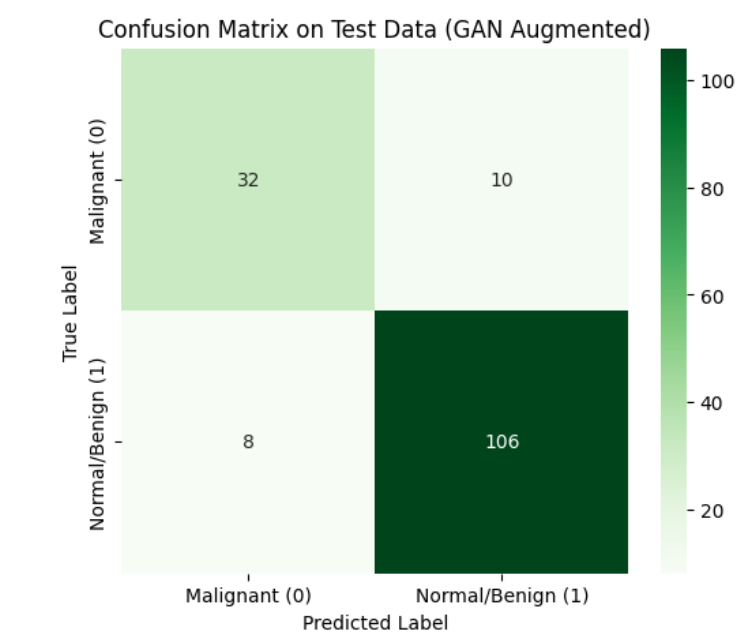
\includegraphics[width=0.6\textwidth]{confusion_matrix_gan.png} 
	\caption{ماتریس آشفتگی مدل \lr{ResNet-18} روی داده‌های تست (پس از افزودن داده‌های \lr{GAN})}
	\label{fig:resnet_gan_cm}
\end{figure}

\vspace{0.5cm}
\textbf{نتیجه‌گیری نهایی تمرین:}

این آزمایش به وضوح اثبات می‌کند که در مسائلی که با محدودیت شدید داده و توزیع نامتوازن کلاس‌ها مواجه هستیم، استفاده از یک شبکه متخاصم مولدِ پایدار و بهینه‌شده (\lr{Stabilized cDCGAN}) برای افزایش داده‌ها (\lr{Data Augmentation})، می‌تواند به طرز مؤثری خطای مدل را در کلاس‌های حیاتی کاهش داده و یک سیستم کمک‌تشخیصی (\lr{CAD}) بسیار قابل‌اعتمادتر ارائه دهد.

%====================================================
%                 QUESTION 2
%====================================================

\section{پرسش ۲: شبکه‌های رمزگذار - رمزگشا مولد }

در این پرسش به بررسی، پیاده‌سازی و مقایسه رویکردهای مختلف کاهش ابعاد و مدل‌های مولد می‌پردازیم. هدف نهایی، درک تفاوت میان روش‌های کلاسیک (مانند \lr{PCA} و \lr{ISOMAP}) و معماری‌های مبتنی بر یادگیری عمیق (مانند \lr{Autoencoder} استاندارد و \lr{Variational Autoencoder}) بر روی یک مجموعه داده تصویری است. با توجه به صورت سوال، از مجموعه داده \lr{CIFAR-10} که شامل تصاویر رنگی ۳۲ در ۳۲ پیکسل است، استفاده خواهد شد.

%----------------------------------------------------
%                 SUBSECTION 2-1
%----------------------------------------------------
\subsection{مجموعه دادگان }

اولین گام در هر پروژه یادگیری ماشین، آماده‌سازی داده‌هاست. مجموعه داده \lr{CIFAR-10} شامل ۶۰,۰۰۰ تصویر رنگی در ۱۰ کلاس مختلف است (۵۰,۰۰۰ داده آموزشی و ۱۰,۰۰۰ داده آزمون). از آنجا که شبکه‌های عصبی با داده‌های نرمال‌شده عملکرد بسیار بهتر و همگرایی سریع‌تری دارند، مقادیر پیکسل‌ها را که در ابتدا بین ۰ تا ۲۵۵ هستند، بر ۲۵۵ تقسیم می‌کنیم تا به بازه استاندارد صفر تا یک منتقل شوند.

\begin{latin}
	\begin{lstlisting}[language=Python, caption={Load and preprocess CIFAR-10 dataset}]
		import numpy as np
		import matplotlib.pyplot as plt
		from tensorflow import keras
		from keras import layers, Model
		from keras.datasets import cifar10
		
		# Load CIFAR-10 dataset
		(x_train, y_train), (x_test, y_test) = cifar10.load_data()
		
		# Normalize pixel values to be between 0 and 1
		x_train = x_train.astype('float32') / 255.0
		x_test = x_test.astype('float32') / 255.0
		
		# Flatten labels from shape (N, 1) to (N,)
		y_train = y_train.flatten()
		y_test = y_test.flatten()
		
		# Print shapes to verify
		print(f"x_train shape: {x_train.shape} - y_train shape: {y_train.shape}")
		print(f"x_test shape:  {x_test.shape} - y_test shape:  {y_test.shape}")
	\end{lstlisting}
\end{latin}

\begin{figure}[H]
	\centering
	
\includegraphics[width=0.7\textwidth]{k1.png}
	\caption{خروجی کد}
\end{figure}
%----------------------------------------------------
%                 SUBSECTION 2-2
%----------------------------------------------------
\subsection{انجام \lr{PCA} و \lr{ISOMAP} }

در این بخش دو روش کلاسیک کاهش ابعاد را مقایسه می‌کنیم:
\begin{itemize}[label=$\bullet$]
	\item \textbf{روش \lr{PCA} (تحلیل مؤلفه‌های اصلی):} این الگوریتم با محاسبه ماتریس کوواریانس داده‌ها و یافتن بردارهای ویژه آن، سیستم مختصات جدیدی می‌سازد که بیشترین واریانس داده‌ها را در کمترین ابعاد ممکن حفظ می‌کند. این روش کاملاً خطی است و سرعت اجرای بسیار بالایی دارد، اما نمی‌تواند الگوهای پیچیده و غیرخطیِ موجود در تصاویر را مدل‌سازی کند.
	\item \textbf{روش \lr{ISOMAP}:} یک رویکرد غیرخطی بر پایه تئوری گراف و یادگیری منیفلد (\lr{Manifold Learning}) است. این الگوریتم ابتدا همسایگان نزدیک هر نقطه را پیدا کرده و یک گراف می‌سازد، سپس کوتاه‌ترین مسیر (فاصله ژئودزیک) بین تمام جفت نقاط را با الگوریتم‌هایی نظیر دایکسترا محاسبه می‌کند و در نهایت با استفاده از \lr{MDS} ابعاد را کاهش می‌دهد. این روش ساختارهای غیرخطی را به خوبی باز می‌کند اما پیچیدگی زمانی آن $O(N^3)$ است که اجرای آن روی داده‌های حجیم مانند \lr{CIFAR-10} نیازمند استخراج یک زیرمجموعه کوچک‌تر است.
\end{itemize}

در کد زیر ابتدا تصاویر سه‌بعدی به بردارهای یک‌بعدی تبدیل شده‌اند. سپس از \lr{RandomizedSearchCV} برای یافتن بهینه‌ترین تنظیمات (Hyperparameters) الگوریتم \lr{KNN} روی فضای کاهش یافته استفاده می‌شود.

\begin{latin}
	\begin{lstlisting}[language=Python, caption={Dimensionality reduction using PCA and ISOMAP, followed by KNN classification}]
		from sklearn.decomposition import PCA
		from sklearn.manifold import Isomap
		from sklearn.neighbors import KNeighborsClassifier
		from sklearn.model_selection import RandomizedSearchCV
		from sklearn.metrics import accuracy_score
		
		# Flatten images: (32, 32, 3) becomes 3072
		x_train_flat = x_train.reshape(len(x_train), -1)
		x_test_flat = x_test.reshape(len(x_test), -1)
		
		# 1. Apply PCA
		pca_components = 64
		pca = PCA(n_components=pca_components)
		x_train_pca = pca.fit_transform(x_train_flat)
		x_test_pca = pca.transform(x_test_flat)
		
		# 2. Apply ISOMAP 
		# Using a random subset of 5000 samples due to high computational complexity
		np.random.seed(42)
		subset_idx = np.random.choice(len(x_train_flat), 5000, replace=False)
		x_train_sub = x_train_flat[subset_idx]
		y_train_sub = y_train[subset_idx]
		
		isomap = Isomap(n_components=pca_components, n_neighbors=5)
		x_train_iso = isomap.fit_transform(x_train_sub)
		x_test_iso = isomap.transform(x_test_flat)
		
		# 3. KNN Classification with Randomized Search on PCA data
		param_grid = {
			'n_neighbors': [3, 5, 7, 11],
			'weights': ['uniform', 'distance']
		}
		
		knn = KNeighborsClassifier()
		random_search = RandomizedSearchCV(
		estimator=knn, 
		param_distributions=param_grid, 
		n_iter=4, 
		cv=3, 
		random_state=42,
		n_jobs=-1
		)
		
		# Fit random search
		random_search.fit(x_train_pca, y_train)
		
		# Evaluate the best model
		best_knn = random_search.best_estimator_
		acc_pca = accuracy_score(y_test, best_knn.predict(x_test_pca))
		print(f"Best KNN Accuracy on PCA Data: {acc_pca:.4f}")
	\end{lstlisting}
\end{latin}
\begin{figure}[H]
	\centering
	
\includegraphics[width=0.7\textwidth]{k2.png}
	\caption{خروجی کد}
\end{figure}

%----------------------------------------------------
%                 SUBSECTION 2-3
%----------------------------------------------------
\subsection{رمزگذار - رمزگشا}

یک \lr{Autoencoder} (خودرمزگذار) یک شبکه عصبی است که هدف آن یادگیری یک نمایش فشرده (فضای نهان یا \lr{Latent Space}) برای داده‌های ورودی است. این شبکه از دو بخش تشکیل شده است:
\begin{enumerate}
	\item \textbf{\lr{Encoder} (رمزگذار):} داده ورودی با ابعاد بالا را گرفته و به یک بردار با ابعاد کمتر فشرده می‌کند. این بخش ویژگی‌های کلیدی داده را استخراج می‌کند.
	\item \textbf{\lr{Decoder} (رمزگشا):} بردار فشرده شده را دریافت کرده و تلاش می‌کند تا داده ورودی اولیه را بازسازی کند.
\end{enumerate}

برای بررسی دقیق‌تر، ما دو معماری مختلف پیاده‌سازی می‌کنیم: معماری \lr{Dense} (کاملاً متصل) که تمام پیکسل‌ها را به صورت مسطح می‌بیند، و معماری \lr{Convolutional} که روابط مکانی و همسایگی پیکسل‌ها را حفظ می‌کند. همچنین شبکه را روی حداقل دو فضای نهان با ابعاد مختلف (مثلاً ۳۲ و ۶۴) بررسی کرده و نتایج آن را به الگوریتم \lr{KNN} می‌سپاریم.

\begin{latin}
	\begin{lstlisting}[language=Python, caption={Standard Autoencoder with Dense and Convolutional architectures}]
		def build_dense_autoencoder(latent_dim):
		# Dense Encoder
		inputs = keras.Input(shape=(32, 32, 3))
		x = layers.Flatten()(inputs)
		x = layers.Dense(512, activation='relu')(x)
		x = layers.Dense(256, activation='relu')(x)
		encoded = layers.Dense(latent_dim, activation='relu')(x)
		
		# Dense Decoder
		x = layers.Dense(256, activation='relu')(encoded)
		x = layers.Dense(512, activation='relu')(x)
		x = layers.Dense(32 * 32 * 3, activation='sigmoid')(x)
		decoded = layers.Reshape((32, 32, 3))(x)
		
		return Model(inputs, encoded), Model(inputs, decoded)
		
		def build_conv_autoencoder(latent_dim):
		# Convolutional Encoder
		inputs = keras.Input(shape=(32, 32, 3))
		x = layers.Conv2D(32, 3, activation='relu', strides=2, padding='same')(inputs)
		x = layers.Conv2D(64, 3, activation='relu', strides=2, padding='same')(x)
		x = layers.Flatten()(x)
		encoded = layers.Dense(latent_dim, activation='relu')(x)
		
		# Convolutional Decoder
		x = layers.Dense(8 * 8 * 64, activation='relu')(encoded)
		x = layers.Reshape((8, 8, 64))(x)
		x = layers.Conv2DTranspose(64, 3, activation='relu', strides=2, padding='same')(x)
		x = layers.Conv2DTranspose(32, 3, activation='relu', strides=2, padding='same')(x)
		decoded = layers.Conv2DTranspose(3, 3, activation='sigmoid', padding='same')(x)
		
		return Model(inputs, encoded), Model(inputs, decoded)
		
		architectures = {
			'Dense': build_dense_autoencoder, 
			'Conv': build_conv_autoencoder
		}
		latent_dimensions = [32, 64]
		
		for arch_name, build_fn in architectures.items():
		for l_dim in latent_dimensions:
		encoder, autoencoder = build_fn(l_dim)
		autoencoder.compile(optimizer='adam', loss='mse')
		
		print(f"Training {arch_name} Autoencoder | Latent Dim: {l_dim}")
		# Train the model (epochs limited for demonstration)
		autoencoder.fit(x_train, x_train, epochs=10, batch_size=256, verbose=0)
		
		# Extract features (dimensionality reduction)
		train_latent = encoder.predict(x_train, verbose=0)
		test_latent = encoder.predict(x_test, verbose=0)
		
		# Classify using KNN
		knn = KNeighborsClassifier(n_neighbors=5)
		knn.fit(train_latent, y_train)
		accuracy = knn.score(test_latent, y_test)
		
		print(f"KNN Accuracy ({arch_name} AE, Latent Dim {l_dim}): {accuracy:.4f}\n")
	\end{lstlisting}
\end{latin}

\begin{figure}[H]
	\centering
	
\includegraphics[width=0.7\textwidth]{k3.png}
	\caption{خروجی کد}
\end{figure}
%----------------------------------------------------
%                 SUBSECTION 2-4
%----------------------------------------------------
\subsection{خود رمزگذار متغیر (\lr{Variational Auto Encoder}) }

شبکه‌های \lr{VAE} یک ارتقاء بنیادی بر روی اتوانکدرهای استاندارد هستند. در حالی که یک اتوانکدر معمولی داده‌ها را به نقاطی ثابت (\lr{Deterministic}) در فضای نهان نگاشت می‌کند که باعث می‌شود فضای نهان گسسته و نامنظم باشد، \lr{VAE} ورودی را به پارامترهای یک توزیع احتمال (معمولاً توزیع نرمال با میانگین $\mu$ و انحراف معیار $\sigma$) مپ می‌کند.

این کار دو مزیت بزرگ دارد: اول اینکه فضای نهان پیوسته و هموار می‌شود و دوم اینکه با نمونه‌برداری (\lr{Sampling}) تصادفی از این فضا، می‌توانیم تصاویر کاملاً جدیدی تولید کنیم (\lr{Generative Model}). برای اینکه در فرآیند نمونه‌برداریِ تصادفی، عملیات پس‌انتشار خطا (\lr{Backpropagation}) دچار مشکل نشود، از تکنیکی به نام \lr{Reparameterization Trick} استفاده می‌شود. تابع زیان (\lr{Loss Function}) در این شبکه ترکیبی از خطای بازسازی تصویر و خطای \lr{KL Divergence} است که وظیفه تنظیم کردن توزیع فضای نهان را بر عهده دارد.

در این بخش نیز مشابه حالت قبل، معماری را یک بار با لایه‌های \lr{Convolutional} و یک بار با لایه‌های \lr{Dense} پیاده‌سازی کرده و در دو ابعاد مختلف تست می‌کنیم.

\begin{latin}
	\begin{lstlisting}[language=Python, caption={Variational Autoencoder (VAE) implementation with Reparameterization trick}]
		import tensorflow as tf
		
		class Sampling(layers.Layer):
		"""Uses (z_mean, z_log_var) to sample z, the vector encoding a digit."""
		def call(self, inputs):
		z_mean, z_log_var = inputs
		batch = tf.shape(z_mean)[0]
		dim = tf.shape(z_mean)[1]
		epsilon = tf.keras.backend.random_normal(shape=(batch, dim))
		# Reparameterization trick
		return z_mean + tf.exp(0.5 * z_log_var) * epsilon
		
		def build_vae_components(architecture, latent_dim):
		inputs = keras.Input(shape=(32, 32, 3))
		
		# 1. Build Encoder
		if architecture == 'Dense':
		x = layers.Flatten()(inputs)
		x = layers.Dense(512, activation='relu')(x)
		x = layers.Dense(256, activation='relu')(x)
		else: # Conv
		x = layers.Conv2D(32, 3, activation='relu', strides=2, padding='same')(inputs)
		x = layers.Conv2D(64, 3, activation='relu', strides=2, padding='same')(x)
		x = layers.Flatten()(x)
		
		z_mean = layers.Dense(latent_dim, name='z_mean')(x)
		z_log_var = layers.Dense(latent_dim, name='z_log_var')(x)
		z = Sampling()([z_mean, z_log_var])
		encoder = Model(inputs, [z_mean, z_log_var, z], name='encoder')
		
		# 2. Build Decoder
		latent_inputs = keras.Input(shape=(latent_dim,))
		if architecture == 'Dense':
		x = layers.Dense(256, activation='relu')(latent_inputs)
		x = layers.Dense(512, activation='relu')(x)
		x = layers.Dense(32 * 32 * 3, activation='sigmoid')(x)
		decoded = layers.Reshape((32, 32, 3))(x)
		else: # Conv
		x = layers.Dense(8 * 8 * 64, activation='relu')(latent_inputs)
		x = layers.Reshape((8, 8, 64))(x)
		x = layers.Conv2DTranspose(64, 3, activation='relu', strides=2, padding='same')(x)
		x = layers.Conv2DTranspose(32, 3, activation='relu', strides=2, padding='same')(x)
		decoded = layers.Conv2DTranspose(3, 3, activation='sigmoid', padding='same')(x)
		
		decoder = Model(latent_inputs, decoded, name='decoder')
		return encoder, decoder
		
		class VAE(keras.Model):
		def __init__(self, encoder, decoder, **kwargs):
		super().__init__(**kwargs)
		self.encoder = encoder
		self.decoder = decoder
		
		def train_step(self, data):
		if isinstance(data, tuple): 
		data = data[0]
		
		with tf.GradientTape() as tape:
		z_mean, z_log_var, z = self.encoder(data)
		reconstruction = self.decoder(z)
		
		# Reconstruction loss (Binary Crossentropy)
		rec_loss = tf.reduce_mean(
		tf.reduce_sum(keras.losses.binary_crossentropy(data, reconstruction), axis=(1, 2))
		)
		# KL Divergence loss
		kl_loss = -0.5 * (1 + z_log_var - tf.square(z_mean) - tf.exp(z_log_var))
		kl_loss = tf.reduce_mean(tf.reduce_sum(kl_loss, axis=1))
		
		total_loss = rec_loss + kl_loss
		
		grads = tape.gradient(total_loss, self.trainable_weights)
		self.optimizer.apply_gradients(zip(grads, self.trainable_weights))
		return {"loss": total_loss, "rec_loss": rec_loss, "kl_loss": kl_loss}
		
		# Global variables to save models for the next subsection
		saved_vae_decoder = None
		saved_z_mean_train = None
		
		for arch in ['Dense', 'Conv']:
		for l_dim in [2, 32]:
		encoder, decoder = build_vae_components(arch, l_dim)
		vae = VAE(encoder, decoder)
		vae.compile(optimizer=keras.optimizers.Adam())
		
		print(f"Training {arch} VAE | Latent Dim: {l_dim}")
		vae.fit(x_train, epochs=10, batch_size=256, verbose=0)
		
		# Use only the mean (z_mean) for representation learning & KNN
		z_mean_train, _, _ = encoder.predict(x_train, verbose=0)
		z_mean_test, _, _ = encoder.predict(x_test, verbose=0)
		
		knn = KNeighborsClassifier(n_neighbors=5)
		knn.fit(z_mean_train, y_train)
		accuracy = knn.score(z_mean_test, y_test)
		
		print(f"KNN Accuracy ({arch} VAE, Latent Dim {l_dim}): {accuracy:.4f}\n")
		
		# Keep the 2D Conv VAE models to plot in the next part
		if arch == 'Conv' and l_dim == 2:
		saved_vae_decoder = decoder
		saved_z_mean_train = z_mean_train
	\end{lstlisting}
\end{latin}

\begin{figure}[H]
	\centering
	
\includegraphics[width=0.7\textwidth]{k4.png}
	\caption{خروجی کد}
\end{figure}
%----------------------------------------------------
%                 SUBSECTION 2-5
%----------------------------------------------------
\subsection{کاوش در فضای \lr{latent} }

یکی از جذاب‌ترین ویژگی‌های \lr{VAE} این است که وقتی مدل را با ابعاد نهان برابر با ۲ آموزش می‌دهیم، می‌توانیم یک سیستم مختصات دوبعدی خطی رسم کرده و نقاط مختلف آن را به \lr{Decoder} بدهیم تا تصاویری با انتقال‌های نرم (\lr{Smooth Transitions}) بین کلاس‌ها تولید کند. در کد زیر یک شبکه \lr{Grid} ایجاد شده و هم‌چنین نمودار پراکندگی (\lr{Scatter Plot}) از داده‌های آموزشی در این فضای دوبعدی ترسیم می‌گردد. کدهای مربوطه برای پشتیبانی از تصاویر رنگی اصلاح شده‌اند.

\begin{latin}
	\begin{lstlisting}[language=Python, caption={Generating a grid of images and scatter plot from the 2D VAE latent space}]
		# --- 1. Grid of generated images (Modified for RGB CIFAR-10) ---
		n = 10
		img_dim = 32 # CIFAR-10 spatial dimension
		scale = 2.0
		
		# Initialize an empty array for the grid. Add 3 for RGB channels.
		figure = np.zeros((img_dim * n, img_dim * n, 3))
		
		# Linearly spaced coordinates for 2D latent space
		grid_x = np.linspace(-scale, scale, n)
		grid_y = np.linspace(-scale, scale, n)[::-1]
		
		for i, yi in enumerate(grid_y):
		for j, xi in enumerate(grid_x):
		# Sample a point from the 2D latent space
		z_sample = np.array([[xi, yi]])
		x_decoded = saved_vae_decoder.predict(z_sample, verbose=0)
		
		# Reshape to image dimensions
		digit = x_decoded[0].reshape(img_dim, img_dim, 3)
		
		# Place the generated image in the grid
		figure[
		i * img_dim : (i + 1) * img_dim,
		j * img_dim : (j + 1) * img_dim,
		:
		] = digit
		
		plt.figure(figsize=(10, 10))
		plt.imshow(figure)
		plt.axis('off')
		plt.title("Grid of Generated CIFAR-10 Images")
		plt.savefig("vae_grid.png", dpi=300, bbox_inches='tight')
		plt.show()
		
		# --- 2. Scatter Plot of Latent Space ---
		plt.figure(figsize=(12, 10))
		scatter = plt.scatter(
		saved_z_mean_train[:, 0], 
		saved_z_mean_train[:, 1], 
		c=y_train, 
		cmap='tab10', 
		s=2, 
		alpha=0.8
		)
		plt.colorbar(scatter, ticks=range(10))
		plt.title("Scatter Plot of Train Data in 2D Latent Space")
		plt.xlabel("Latent dimension 1 (z[0])")
		plt.ylabel("Latent dimension 2 (z[1])")
		plt.savefig("vae_scatter.png", dpi=300, bbox_inches='tight')
		plt.show()
	\end{lstlisting}
\end{latin}

در قسمت زیر جایگاه قرارگیری خروجی کدها (عکس‌های تولید شده) تعبیه شده است. پس از اجرای کد پایتون و تولید تصاویر \lr{vae\_grid.png} و \lr{vae\_scatter.png}، دستورات \lr{includegraphics} مربوطه را از حالت کامنت خارج کنید.

\begin{figure}[H]
	\centering
	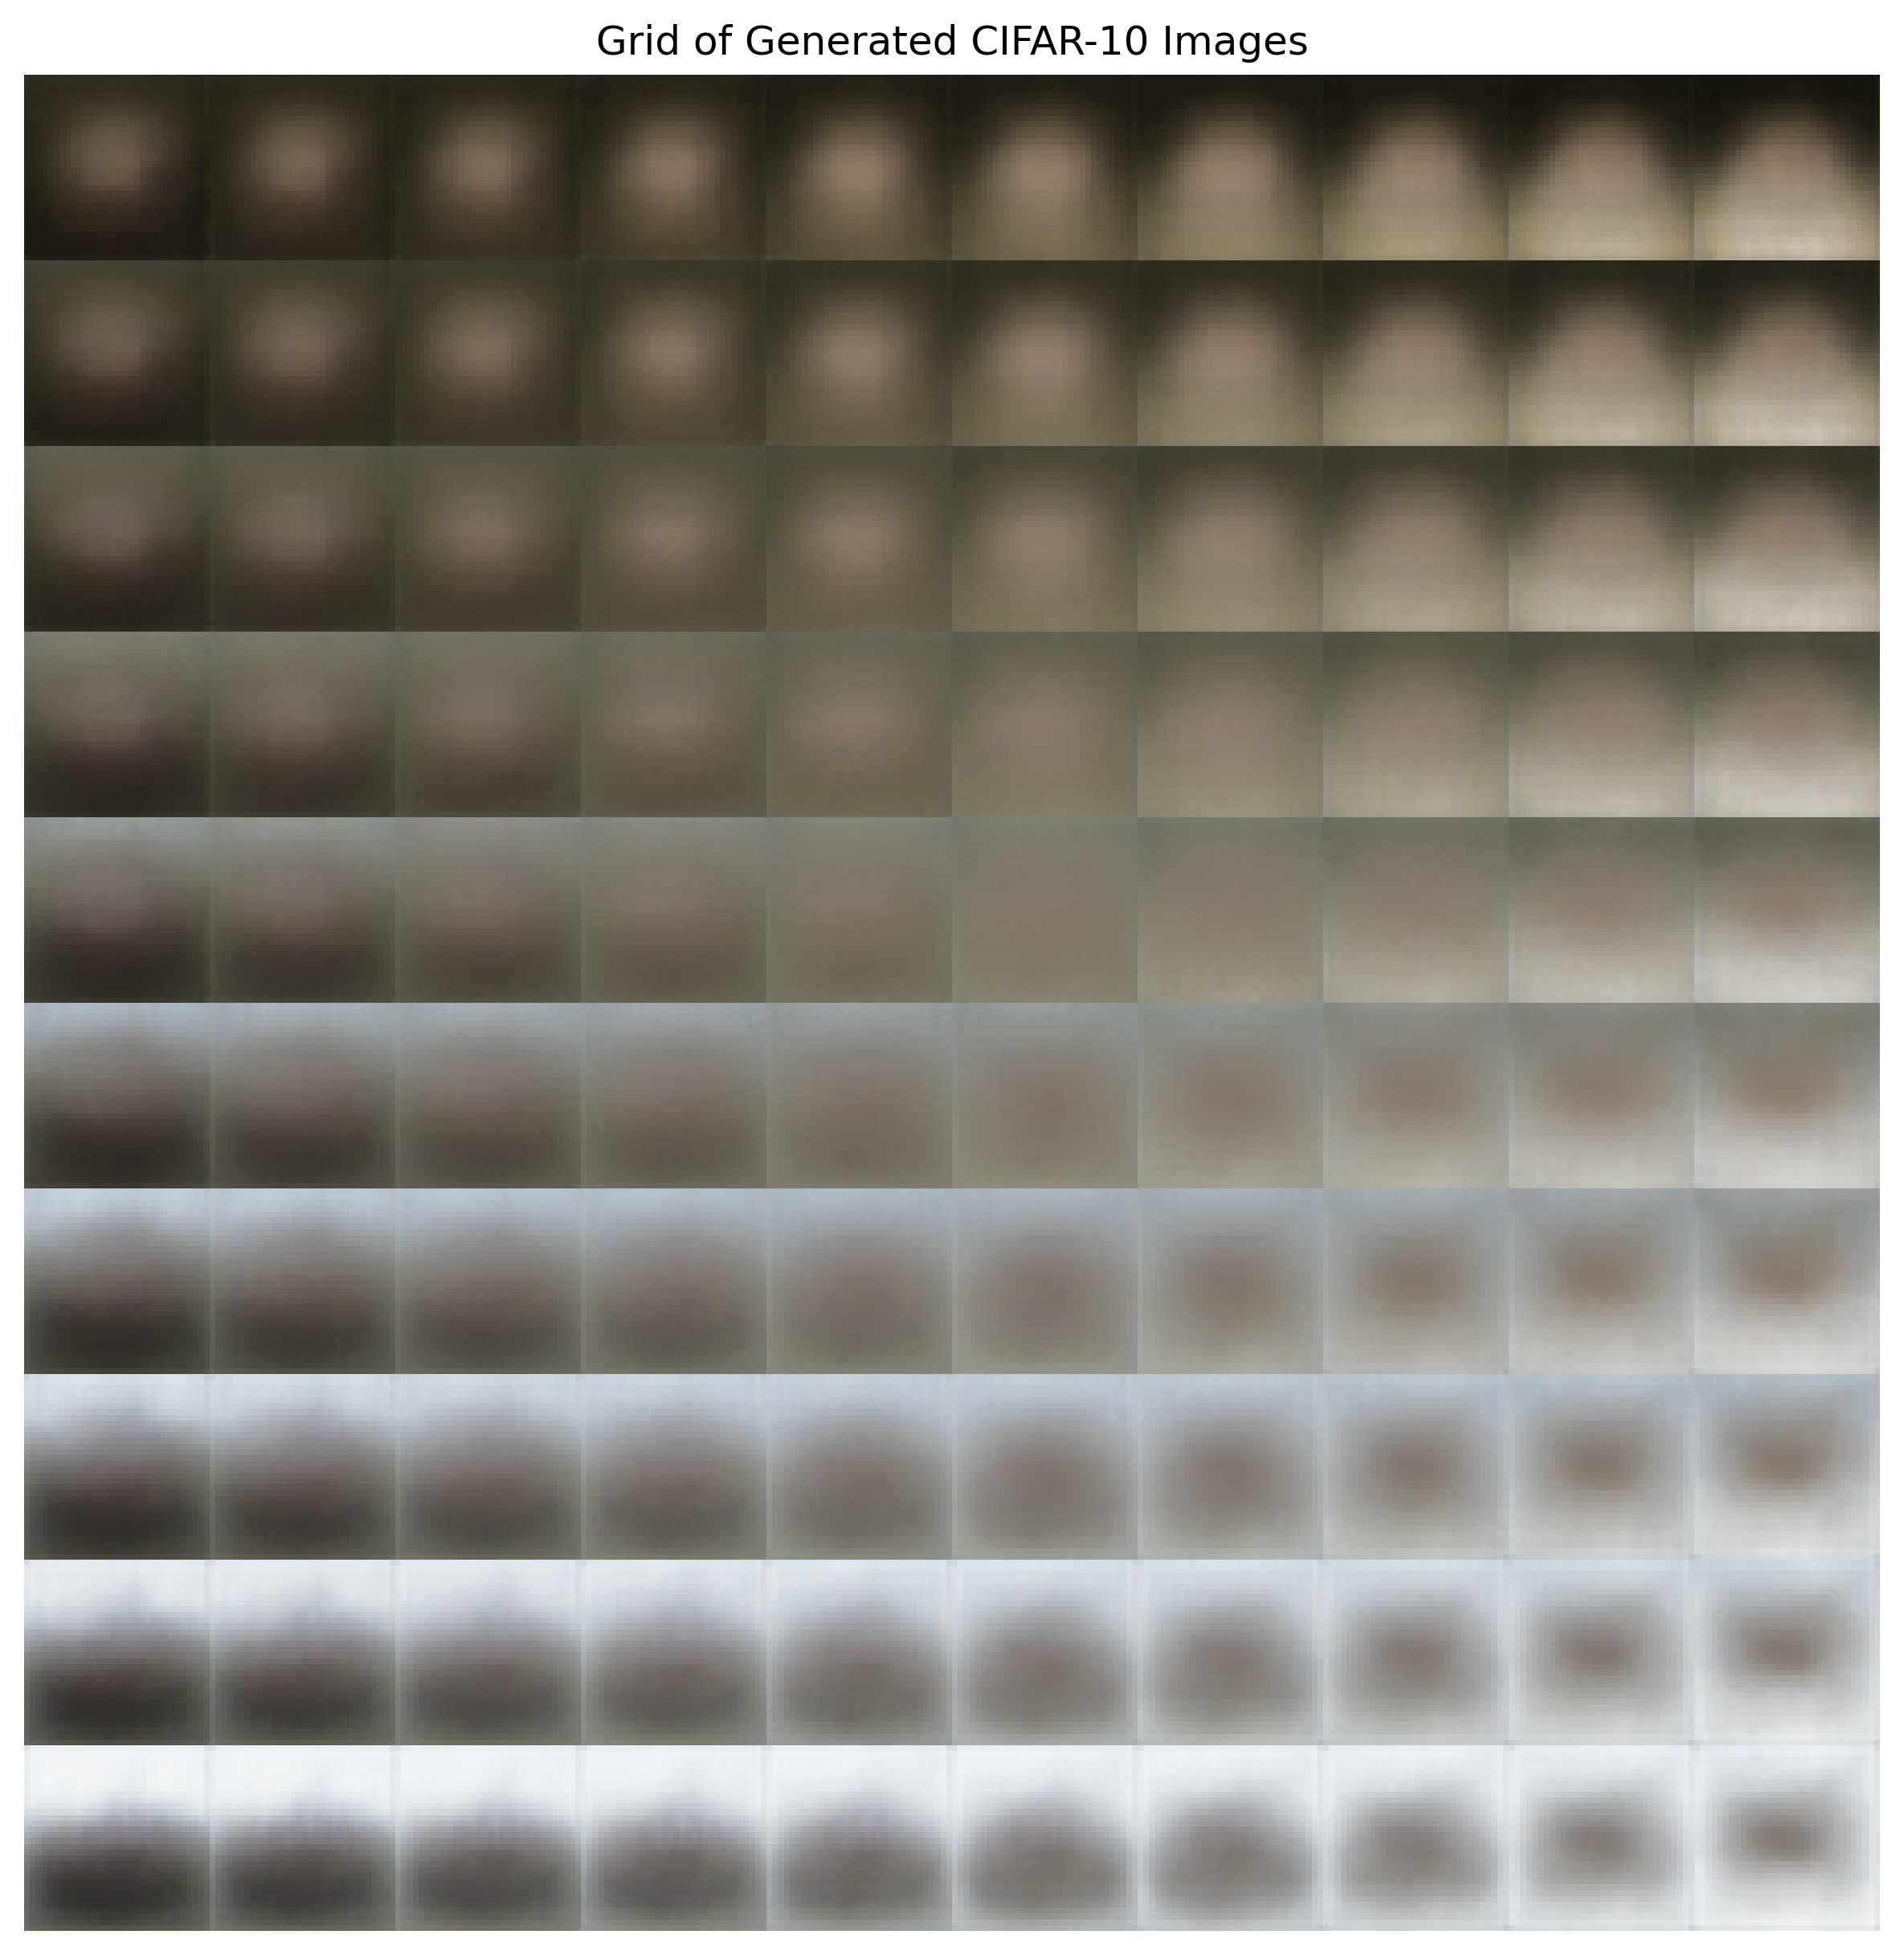
\includegraphics[width=0.55\textwidth]{vae_grid.png}
	\caption{نمونه تصاویر \lr{CIFAR-10} تولید شده از مختصات شبکه \lr{Grid} توسط \lr{Decoder}}
\end{figure}

\begin{figure}[H]
	\centering
	 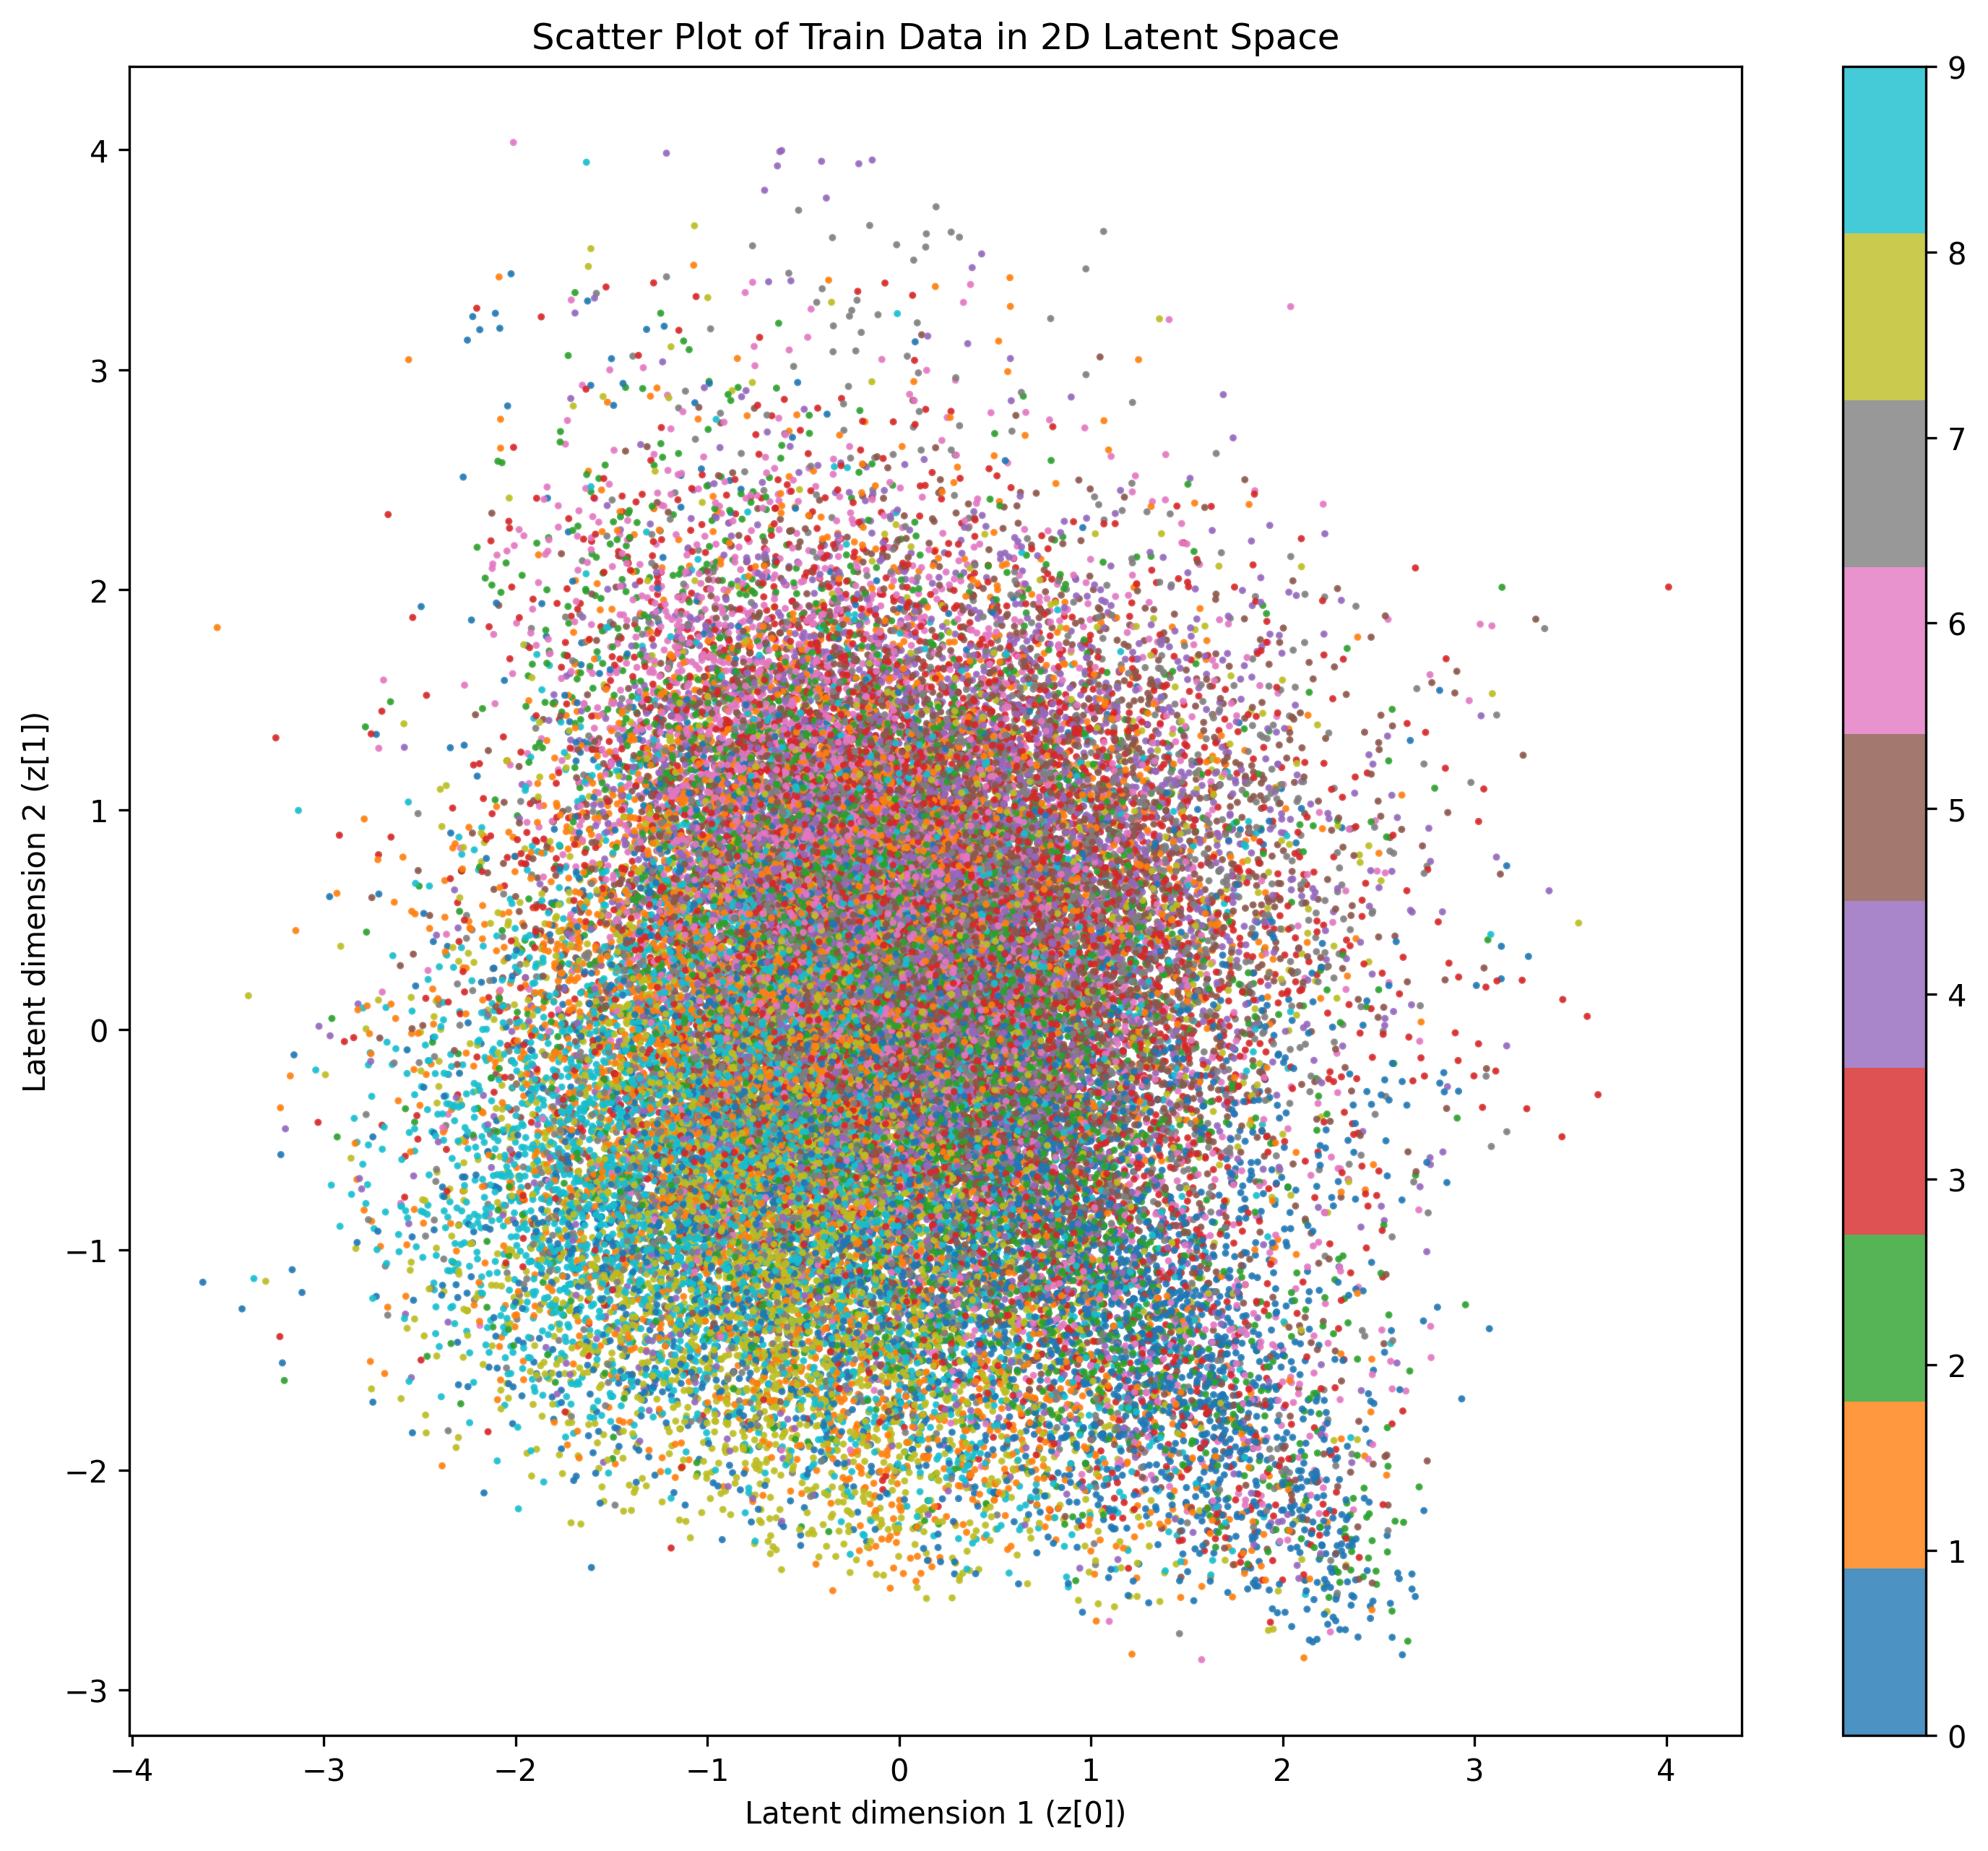
\includegraphics[width=0.65\textwidth]{vae_scatter.png}
	\caption{نمودار پراکندگی (\lr{Scatter Plot}) داده‌های آموزشی در فضای نهان دوبعدی \lr{VAE}}
\end{figure}

%----------------------------------------------------
%                 SUBSECTION 2-6
%----------------------------------------------------
\subsection{مدل‌های انتشار (\lr{Diffusion Models}) }

مدل‌های انتشار (\lr{Diffusion Models}) نسل جدیدی از شبکه‌های مولد عمیق هستند که امروزه پشتوانه بسیاری از ابزارهای قدرتمند تولید تصویر (مانند \lr{Midjourney} و \lr{DALL-E 3}) می‌باشند. این مدل‌ها فرآیند تولید داده را با الهام از علم ترمودینامیک و فیزیک آماری انجام می‌دهند و شامل دو فرآیند اصلی هستند:
\begin{enumerate}
	\item \textbf{فرآیند رفت (\lr{Forward/Diffusion Process}):} در این مرحله بر اساس یک زنجیره مارکوف (\lr{Markov Chain})، به صورت گام‌به‌گام و تحت زمان $t$، نویز تصادفی گاوسی به تصویر واقعی اضافه می‌شود تا جایی که پس از مثلاً ۱۰۰۰ مرحله، تصویر کاملاً به یک نویز خالص تبدیل شود و هیچ اثری از داده اولیه باقی نماند.
	\item \textbf{فرآیند برگشت (\lr{Reverse/Denoising Process}):} مدل یاد می‌گیرد تا این فرآیند تخریب را معکوس کند. یک شبکه عصبی (به طور معمول معماری \lr{U-Net} دارای اتصالات پرشی) آموزش می‌بیند که با گرفتن نویز خالص در مرحله $T$، آن را در مراحل متوالی نویززدایی کند و در نهایت به یک تصویر کاملاً جدید و واضح برسد.
\end{enumerate}

\textbf{مقایسه عملکرد و معماری با \lr{VAE}:}
\begin{itemize}[label=$\bullet$]
	\item \textbf{وضوح و کیفیت تصویر:} نقطه ضعف بزرگ \lr{VAE}ها استفاده از تابع زیان میانگین مربعات خطا (\lr{MSE}) برای بازسازی پیکسل‌ها است. این کار باعث می‌شود خروجی این شبکه‌ها تمایل به مات شدن (\lr{Blurriness}) داشته باشد. اما در مدل‌های انتشار، به دلیل اینکه شبکه مستقیماً نویز را تخمین می‌زند و گام‌به‌گام آن را حذف می‌کند، خروجی‌ها بسیار شفاف، واضح و واقع‌گرایانه (\lr{High Fidelity}) هستند.
	\item \textbf{سرعت استنتاج (\lr{Inference Speed}):} شبکه‌های \lr{VAE} بسیار سریع هستند، زیرا با دادن یک بردار نویز تصادفی به \lr{Decoder} تنها با یک فورواردپس (\lr{Single-step}) تصویر تولید می‌شود. در مقابل، مدل‌های \lr{Diffusion} بسیار کند هستند و نیازمند ده‌ها یا صدها حلقه تکرار در شبکه عصبی برای رسیدن به تصویر نهایی می‌باشند.
	\item \textbf{فضای نهان:} شبکه‌های \lr{VAE} ذاتا یک فضای نهان بسیار فشرده (\lr{Low-Dimensional Bottleneck}) و دارای نظم معنایی تولید می‌کنند که برای تسک‌های مهندسی ویژگی (\lr{Feature Extraction}) ایده‌آل است. اما مدل‌های انتشار کلاسیک فضای نهانی هم‌اندازه با خود تصویر اصلی دارند (مگر در مدل‌های ترکیبی نوین مانند \lr{Latent Diffusion} که فرآیند پخش را درون فضای نهانِ یک \lr{Autoencoder} انجام می‌دهند).
\end{itemize}
%----------------------------------------------------
%                 SUBSECTION 2-7 (Conclusion)
%----------------------------------------------------
\subsection{جمع‌بندی و نتیجه‌گیری نهایی}

با بررسی و پیاده‌سازی روش‌های مختلف کاهش ابعاد و مدل‌های مولد بر روی مجموعه داده \lr{CIFAR-10}، می‌توانیم به یک درک جامع از روند تکامل این الگوریتم‌ها دست پیدا کنیم. تحلیل نتایج به‌دست‌آمده را می‌توان در محورهای زیر خلاصه کرد:

\textbf{۱. مقایسه رویکردهای خطی و غیرخطی در کاهش ابعاد:} 
روش \lr{PCA} به عنوان یک رویکرد خطی، سرعت اجرای بسیار بالایی دارد و توانست با حفظ مؤلفه‌های اصلی، به دقت قابل قبولی (حدود ۴۰ درصد با \lr{KNN}) برسد. با این حال، \lr{PCA} از درک روابط پیچیده و غیرخطی درون تصاویر عاجز است. در مقابل، روش \lr{ISOMAP} ساختارهای غیرخطی را بهتر مدل می‌کند، اما پیچیدگی محاسباتی آن مانع از کاربرد عملی آن روی دیتاست‌های حجیم تصویری می‌شود.

\textbf{۲. اهمیت معماری در شبکه‌های عصبی (\lr{Dense} در برابر \lr{Conv}):}
در هر دو شبکه \lr{Autoencoder} استاندارد و \lr{VAE}، مشاهده کردیم که معماری مبتنی بر کانولوشن (\lr{Convolutional}) عملکرد بسیار بهتری نسبت به لایه‌های کاملاً متصل (\lr{Dense}) دارد. لایه‌های \lr{Dense} با مسطح کردن (\lr{Flatten}) تصویر در همان گام اول، تمام اطلاعات مکانی و همسایگی پیکسل‌ها را از بین می‌برند، در حالی که فیلترهای کانولوشنی این ساختار فضایی را حفظ کرده و ویژگی‌های بسیار غنی‌تری استخراج می‌کنند (رسیدن به بالاترین دقت یعنی حدود ۴۲.۸ درصد در \lr{Conv VAE} با بعد ۳۲).

\textbf{۳. چالش ابعاد در فضای نهان (\lr{Latent Space}):}
نتایج نشان داد که فشرده‌سازی بیش از حد اطلاعات (مانند استفاده از بعد نهان برابر با ۲) منجر به افت شدید دقت (تا حدود ۱۶ درصد) می‌شود. در فضای دوبعدیِ \lr{VAE}، به دلیل اعمال تابع زیان \lr{KL Divergence}، کلاس‌های مختلف به شدت روی هم قرار می‌گیرند (هم‌پوشانی در توزیع نرمال حول صفر) و تفکیک‌پذیری از بین می‌رود. اما با افزایش این فضا به ۳۲ بُعد، شبکه ظرفیت کافی برای جداسازی معنایی کلاس‌ها پیدا می‌کند.

\begin{tcolorbox}[
	colback=softpink,
	colframe=softred,
	title=نتیجه نهایی و مسیر پیش‌رو,
	fonttitle=\bfseries\Large,
	coltitle=white
	]
	در نهایت، گذار از \lr{Autoencoder}های استاندارد به \textbf{\lr{VAE}} و سپس به \textbf{\lr{Diffusion Models}} نشان‌دهنده یک تغییر پارادایم در مدل‌های مولد است:
	\begin{itemize}[label=$\bullet$]
		\item \textbf{\lr{Autoencoder}:} فضایی گسسته می‌سازد که صرفاً برای فشرده‌سازی و کاهش ابعاد مناسب است و قابلیت تولید تصویر جدید ندارد.
		\item \textbf{\lr{VAE}:} با تحمیل یک توزیع احتمالاتی، فضایی پیوسته ایجاد می‌کند که قابلیت تولید تصویر دارد، اما به دلیل استفاده از خطای \lr{MSE} در بازسازی، تصاویر نهایی تار (\lr{Blurry}) و فاقد جزئیات دقیق هستند.
		\item \textbf{\lr{Diffusion Models}:} با جایگزینی رویکرد بازسازی مستقیم با فرآیند «نویززدایی گام‌به‌گام»، محدودیت‌های \lr{VAE} را دور زده و تصاویری با بالاترین کیفیت و وضوح ممکن تولید می‌کنند؛ هرچند این کیفیت بالا به بهای افزایش شدید زمان محاسبات (\lr{Inference Time}) تمام می‌شود.
	\end{itemize}
\end{tcolorbox}
\end{document}